\documentclass[../main.tex]{subfiles}



\begin{document}

We take a brief segue to provide some theory into the tail approximation to the $\alpha$-stable distribution that will be useful in the later sections. 

When $\alpha < 2$, the tails of the \asd are are asymptotically equivalent to a Pareto law. More precisely, if $\lambda$ is a standardized $\alpha$-stable variable $\lambda \sim S_\alpha(\sigma, \beta, \mu)$ with $0 < \alpha < 2$, $\sigma = 1$, $\mu = 0$ then as $\lambda \rightarrow \infty$ (\cite{samoradnitsky2017stable}):

\begin{equation}
	\lim_{x \rightarrow \infty} P(\lambda > x) = C_\alpha (1+\beta) x^{-\alpha}
	\label{eq:2__1__1__tail_cdf}
\end{equation}

where: 

\begin{equation*}
	C_\alpha = \left( 2\int_{0}^{\infty} x^{-\alpha} \sin x dx \right)^{-1} = \frac{1}{\pi}\Gamma(\alpha)\sin(\frac{\alpha \pi}{2})
\end{equation*}

We can then differentiate \autoref{eq:2__1__1__tail_cdf} to obtain the pdf of the tail approximation: 

\begin{align}
	\lim_{x \rightarrow \infty}S_\alpha(\lambda = x | \sigma = 1, \beta, \mu = 0) &= f_{pareto}(\lambda = x | \alpha, \beta) \notag \\
	&=  \alpha C_\alpha (1+\beta) x^{-\alpha - 1}
\end{align}

\textbf{Numerical accuracy of the tail approximation}

We first define a metric for the absolute relative error in the tail approximation: 

\begin{equation}
	\epsilon_{rel}(x) =  \left| \frac{ S_\alpha(\lambda = x | 1, \beta, 0) - f_{pareto}(\lambda = x | \alpha, \beta) }{S_\alpha(\lambda = x | 1, \beta, 0)  } \right|
\end{equation}

We can then investigate the numerical accuracy of the tail approximation for $\beta = 1$ and $\alpha < 1$ using Figure \ref{fig:2__1__1__tail_approx}. As expected, we note that the relative error in the tail approximation decreases monotically. 

Note that for $\alpha<1$, there is no clear dependence on the value of $\alpha$ and the rate of convergence of the \asd to the paretian tail approximation.

\begin{figure}[h!]
	\centering
	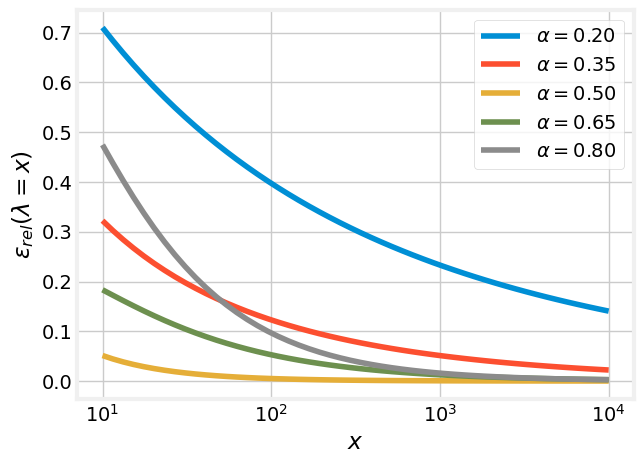
\includegraphics[width=12.0cm]{../plots/2__1__1__tail_approx.png}
	\caption{Relative error in the tail approximation $\epsilon_{rel}(x)$ for $\beta = 1$ and $\alpha < 1$}
	\label{fig:2__1__1__tail_approx}
\end{figure}

\textbf{Sampling from the paretian tail}

Using the paretian tail approximation to the \asd, we note that up to a certain scale parameter($\alpha (1+\beta) C_\alpha$), sampling from a left-truncated $\alpha$-stable distribution can be approximated by sampling from a left-truncated pareto distribution. 

For a left-truncated pareto distribution $f_{pareto}(x | \alpha, \beta)$ lower bounded by $x \geq L$, we the corresponding PDF $f_{bounded \text{ }pareto}(x | \alpha, \beta, L)$ is given by \autoref{eq:2__1__1__bounded_pareto}:

\begin{equation}
	f_{bounded \text{ }pareto}(x | \alpha, \beta, L) =  \alpha L^\alpha \left(\frac{x}{\alpha (1+\beta) C_\alpha}\right)^{-\alpha -1} \label{eq:2__1__1__bounded_pareto}
\end{equation}

We can then sample from this left-truncated pareto distribution easily using the inverse transform method. 

\begin{equation}
x = \alpha (1+\beta) C_\alpha \left( \frac{1-U }{L^\alpha} \right) ^ {-\frac{1}{\alpha}}  \qquad \text{where: } U \sim \text{Unif}(0,1)
\label{eq:2__2__2__bounded_pareto}
\end{equation}

Following \autoref{eq:2__2__2__bounded_pareto}, $x$ will be left-truncated pareto distributed according to $f_{bounded \text{ }pareto}(x | \alpha, \beta, L)$ 
	
\end{document}